\section{ADIOS I/O Abstraction}
\label{sec:adios}

A parallel application that produces data uses ADIOS to define \emph{variables} ($n$-dimensional distributed arrays of a particular type) and \emph{attributes} (labels associated with individual variables or the entire output data set).
It also specifies when the data is available for output. The output is organized around output \emph{Steps}, instead of individual variables.
A Step includes all the variables and attributes that are to be sent to the target at once.
There is nothing in the ADIOS interface that prescribes how to handle the data (e.g. data aggregation among the processes, targeting a single file or one file per process, handling multiple readers, and handling the disappearance of a potential reader).
These belong to the \emph{IO strategy} and are implemented in various ways by different Engines.
The user can control the behavior of the application by choosing a specific engine, and parameterizing it with available options. 

Similarly, a reading application only declares what data it wants to retrieve from a source, each process of the parallel application declaring what it needs, and when it expects the data to be in its memory.
The input is also organized around Steps, not individual variables, which makes the interface a bit more complicated, but it allows for ADIOS to ensure that a reader never gets into an inconsistent state where portion of the data of some variables belong to a certain step, and other portion to another step. 

ADIOS provides a number of engines for movement of data, which are described below.
\todo{Verify this is accurate and complete}

\begin{itemize}
\item \textbf{BPFile}. The default engine for storage I/O. The output file target is a directory, which contains some data files and metadata files. The number of files is tailored to the capability of the file system, not to the number of writers or readers. This ensures scalable I/O performance. The steps stored in a single file target, can be read by other applications step-by-step simultaneously. Therefore, this engine can be used for in situ processing through the file system. 

\item \textbf{HDF5}. This engine can be used to write and read HDF5 formatted files. It uses the Parallel HDF5 library, so it provides only a compatibility layer to process HDF5 files in an ADIOS application workflow but it is only as scalable as the HDF5 library itself. Streaming access to data is not currently available, but will be available once supported by HDF5.

\item \textbf{SST} (Scalable Staging Transport). The most versatile and flexible staging engine uses either RDMA, TCP, UDP, or shared memory to move data from a producer (parallel application) to other consumers (multiple independent parallel applications). Consumers can come and go dynamically without affecting the producer. The output step is buffered in the producer's memory, and readers pull out portions of the buffered data with RDMA operations or talk to a thread in the producer to receive it via TCP. The requirement of all engines to always provide a consistent view of a step to a reader may result in blocking the producer from progressing if the consumer is slower than the producer. The SST writer engine aggregates metadata for every single step, and shares it with all readers. Readers then issue remote reading operations based on the I/O pattern in metadata. This allows the I/O pattern to vary over time. SST also allows readers to disconnect and reconnect while writers keep writing.
To address different application requirements, the SST buffering policy can be configured at run-time. This includes keeping only the most recent step, buffering a fixed window of consecutive steps, or blocking until the step is consumed. In cases where strong coupling is required between applications, the buffer limit can be set to $1$, which ensures that every step is consumed by the reader before the producer moves to the next data step.
For use cases like interactive visualization, buffering only the latest step is useful since the user typically does not want to block the simulation while a particular time step is explored.
While SST aims to provide the flexibility for addressing various application requirements, the fact that it manages metadata for every single step may be overkill for uses cases where the metadata does not change frequently, or at all.

\item \textbf{Insitu-MPI}. This engine is similar to the SST engine, but is motivated by use cases where the metadata is constant across the workflow and a single metadata aggregation at the first data step suffice. After this first step, each writer and reader knows the exact I/O pattern and direct communication is performed using send and receive operations using the MPI world communicator. Because of this, the producer and consumer applications must be launched within a single mpiexec command using the Multiple Program Multiple Data (MPMD) mode.
For very large applications with constant I/O patterns, the Insitu-MPI engine can provide CPU savings for metadata management. However, since it must be launched in MPMD mode under MPI, the flexibility of readers dynamically join or leave is not supported at run-time.
\todo{simplify io pattern.  assumes fixed exchange of data: doesn’t change. Fixed communication pathways. ADIOS is lost.  Don’t mention impleementation what dios does.}

\item \textbf{SSC} (Staging for Strong Coupling).
The SSC engine is also designed for applications that have constant metadata over time. Similar to the Insitu-MPI engine, the SSC engine aggregates metadata once on the first time step. The main difference between SSC and Insitu-MPI is that SSC uses one-sided MPI communication.
The one sided MPI paradigm does not require the send and receive calls to be paired. Instead, it allows direct access to remote memory of another process. This makes it possible for applications to very quickly, and frequently exchange data.
In very large scale coupling use cases this saves the overhead of one side waiting for the other side to complete the send and receive pair. 
\todo{see comment above in IMPI}

\item \textbf{DataMan}. This engine focuses on providing good bandwidth over wide-area-networks. It uses the publish and subscribe communication mechanism of the ZeroMQ library and has been optimized specifically for long-distance low-latency data movement. Unlike other staging engines, such as SSC described above, DataMan does not guarantee that every data step is transferred. Instead, the subscriber is designed to read only the latest data steps, while ignoring the older. This saves the two-way communications for checking step completeness, which usually means several hundred milliseconds in inter-continental data transfers. Because of this, the data transfer latency is greatly reduced and can support near-real-time analysis better than other engines in a wide area network case.

\end{itemize}

\subsection{Discussion of Engine Characteristics}
\begin{figure}[b]
\sidecaption
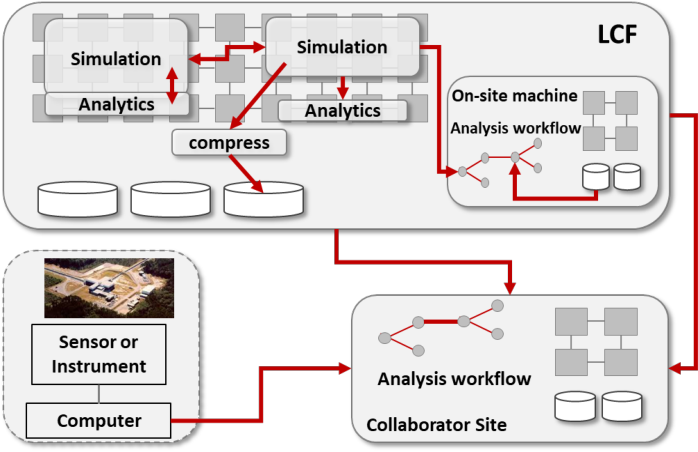
\includegraphics[scale=.75]{figures/ExampleWorkflow.pdf}
\caption{Example workflow using ADIOS in a number of ways. NEEDS to be edited..}
\label{fig:example_workflow}
\end{figure}

The number of engines available in ADIOS provides a large amount of flexibility when selecting a configuration. Further, multiple executables can be connected using the read/write API of an ADIOS engine to support a range of different types of workflows. The example workflow in Figure~\ref{fig:example_workflow} shows a simulation using ADIOS engines to transfer data in a number of different ways. \todo{Dave: Finish this....}

There are a number of factors to consider when deciding which ADIOS engine to use. First and foremost, the choice of engine may depend on a future use case for the data, such as post hoc analysis. In this case, the engine can save data using either the BPFile or HDF5 file formats. For other cases, a number of factors should be considered when choosing the most appropriate engine.

One method to aid in choosing the most appropriate engine for a given scenario is by using a set of empirical and speculative comparison factors~\cite{Kress-isav15}. These comparison factors allow the three classes of engines (file based, in-line based, and in-transit based) to be classified and evaluated. \todo{talk about fault tolerance} Below we list six of the most relevant these comparison factors, and explore the strengths and weaknesses of the different classes of ADIOS engines in relation to those factors. By understanding the strengths and weaknesses of each engine type, it will be possible to make an informed choice of engine selection based the needs of a given use case.

\paragraph{\emph{Data Access:}}
Data access is defined as the ability to access the full breadth of a simulations data, and is also concerned with both the temporal fidelity and temporal range of available data.
\begin{itemize}
    \item \emph{File based methods} generally do not have great data access in terms of data breadth and temporal fidelity. That is, it is generally too expensive to save out all of a simulations state, so data are first culled before being written to disk, while also often skipping many time steps between writes. However, these methods do have the best temporal range, as it is trivial to scan forward or backward in time in a file.
    
    \item \emph{In-line methods} have very good data access. Since the visualization is running on the same node where the data are being generated, they generally have access to all of the simulations data. This also means that they have good temporal fidelity, as they can conceptually operate on every simulation time step. However, in-line methods generally have poor temporal range. This is because once a time step has passed, the visualization routine would have to store it in memory in order to access it later. That said, the available temporal range can be modified by the user depending on how much memory they are willing to devote to storing past time steps. 
    
    \item \emph{In-transit methods} can have very good data access. This access however, depends on how much data a user is willing to send across the network to the in-transit methods. Generally, this is not everything that the simulation produces, so visualization routines may be more limited in this setting. Temporal fidelity can also be very good with in-transit, as every step can be gathered from the simulation if needed. However, these methods suffer the same temporal range issues as in-line methods, where range is user and system dependent.
\end{itemize}
\textbf{Table sub categories:} spatial access, temporal access, temporal range
\begin{itemize}
    \item File: - - +
    \item Inline: + + -
    \item Intransit: 0 0 0 (???)
\end{itemize}

\paragraph{\emph{Data Movement:}}
Data movement is defined as the amount of data being sent from a simulation process. That data can either be sent to disk, to another node in the simulations allocation, or a separate allocation entirely. 
\begin{itemize}
    \item \emph{File based methods} suffer the most in terms of data movement. Writing data to disk is a slow operation, and writing large amounts of data can stall a simulation for large periods of time. 
    
    \item \emph{In-line methods} data movement can can range from none, to simulation stalling levels. This is because some visualization algorithms traditionally require large amounts of inter-node communication which can be enormously expensive compared to a smaller node allocation. \todo{does this go in scalability?}
    
    \item \emph{In-transit methods} have a different issue with regards to data movement. Before visualization can take place, the data must be sent from the simulation to a visualization resource for processing. This dump from the simulation to the visualization resource has the potential to cause network interference or even slowdown the simulation while data is sent. However, this data transmission has potential to end up moving far less data, in total, than in-line visualization. This is due to the amount of inter-node communication that takes place during communication heavy visualization routines, meaning that in-transit will have to send less data since they typically operate on smaller allocations.
\end{itemize}
\textbf{Table sub categories:} None
\begin{itemize}
    \item File: -
    \item Inline: +
    \item Intransit: 0
\end{itemize}

\paragraph{\emph{Scalability:}}
Scalability is defined as the ability of a visualization and analysis task to efficiently utilize the resources it is given.
\begin{itemize}
    \item \emph{File based methods} 
    
    \item \emph{In-line methods} are constrained to running on the full allocation of the simulation. While this level of concurrency can be advantageous for embarrassingly parallel algorithms that perform little synchronization or communication, it can be a bottleneck for routines that require significant communication (e.g. particle advection), or algorithms that don't scale up to the levels of simulation codes (e.g. hundreds of thousands of cores).
    
    \item \emph{In-transit methods} have the benefit that the visualization resource can be appropriately configured for the tasks to be performed.  Algorithms that require significant synchronization and communication will generally perform much better at lower levels of concurrency, and this can be used to optimize the performance.
\end{itemize}
\textbf{Table sub categories:} I/O, compute-heavy, comm-heavy
\begin{itemize}
    \item File: - 0 0
    \item Inline: + + -
    \item Intransit: 0 + +
\end{itemize}

\paragraph{\emph{Coordination:}}
Coordination is defined as the need for a visualization and analysis task to coordinate with the state of the simulation. This factor is concerned with such items as ensuring data is moved and available for use, how to handle missing or incomplete data, and what to do if visualization resources are not available. 
\begin{itemize}
    \item \emph{File based methods} require no coordination.
    
    \item \emph{In-line methods} require minimal coordination. If visualization code is embedded in the simulation, coordination is as the visualization routine at the end of the simulation main loop. For production tools like LibSim and Catalyst the coordination is very similar, but the call is made into the particular library.
    
    \item \emph{In-transit methods} require much more coordination. At every simulation cycle where visualization needs to be performed calls must be made to transfer the data to the visualization resource. This transfer requires use of the network and coordination on both the sending and receiving side to ensure the data are successfully sent and received. This method also has a particular pitfall in that the visualization resource may not available for some reason to receive data, meaning the sender has to have rules about how to proceed in this case.
\end{itemize}

\textbf{Table sub categories:} None?
\begin{itemize}
    \item File: +
    \item Inline: +
    \item Intransit: -
\end{itemize}

\paragraph{\emph{Resource Requirements:}}
Resource Requirements is defined as the additional resources that a visualization and analysis task needs in order to execute.
\begin{itemize}
    \item \emph{File based methods} use the simulations resources to write the data to disk, so no extra resources are required to save the data. These methods do however require extra resources when the data is analyzed after the simulation is complete. The amount of resources need to do this analysis can vary depending on the required task. 
    
    \item \emph{In-line methods} share the simulation resources with the visualization routines. This coexistence can have negative implications for the simulation of the visualization routines require large amounts of memory or communication, which can add to the simulations cost. Therefore simulations will generally dedicate a fixed window of time for visualization, while placing restrictions on memory or even network use.
    
    \item \emph{In-transit methods} by definition require additional resources, adding those resources as extra cost to a running simulation. However, these additional resources can be used asynchronously once the data are transferred, allowing the simulation to proceed after transmitting data. Special care must be taken to allocate the right amount of resources for the visualization task at hand, or the resources might not be ready the next time the simulation is ready to send data.
\end{itemize}

\textbf{Table sub categories:} Use sim resources, use extra resources
\begin{itemize}
    \item File: 0 -
    \item Inline: - +
    \item Intransit: 0 -
\end{itemize}

\paragraph{\emph{Exploratory Visualization:}}
Exploratory Visualization is defined as the ability to visually sift through data coming from the simulation in order to find features of interest.
\begin{itemize}
    \item \emph{File based methods} can have access to the full spatio-temporal data from the simulation, but generally only have access to subsets of data, or very sparse temporal data. File based methods though have the benefit of not blocking the simulation, and the data can be explored and visualized for as long as needed.

    \item \emph{In-line methods} have access to the full range of spatio-temporal data from the simulation. The downside of this method for exploratory visualization is that the exploration will come at the cost of pausing the simulation while a time step is explored interactively.
    
    \item \emph{In-transit methods} can have access to the full spatio-temporal range of the simulation, but are generally more restricted, and only receive a subset of the full simulation state. However, this method has the benefit of being able to perform exploratory visualization while not blocking the simulation, since the simulation can proceed asynchronously while a given time step is explored.
\end{itemize}
\textbf{Table sub categories:} spatio-temporal access, block simulation
\begin{itemize}
    \item File: + + (?)
    \item Inline: + -
    \item Intransit: 0 +
\end{itemize}

\paragraph{\emph{Fault Tolerance:}}
Fault Tolerance is defined as a methods resilience to causing an irrecoverable problem for the simulation, causing it to crash. 

\begin{itemize}
    \item \emph{File based methods} are very resilient to faults.
    
    \item \emph{In-line methods} can have significant issues with fault tolerance. This is because the visualization and simulation run together on the same resource, and the visualization can expose the simulation to data corruption, infinite loops, or errors from visualization routines.
    
    \item \emph{In-transit methods} are inherently more fault tolerant because of the clear and distinct separation between the simulation and the visualization resources and binaries. In this paradigm the data transfer to the visualization resource becomes the main point of exposure to faults.
\end{itemize}
\textbf{Table sub categories:} None
\begin{itemize}
    \item File: +
    \item Inline: -
    \item Intransit: +
\end{itemize}


\begin{table}
\centering
\caption{Table caption}
\label{table:comparisonFactors}
\renewcommand{\arraystretch}{1.5}
\setlength{\tabcolsep}{8pt}
\begin{tabular}{
>{\columncolor[HTML]{EFEFEF}}c |ccc}
\hline
\multicolumn{1}{l|}{\cellcolor[HTML]{EFEFEF}} & \multicolumn{3}{c}{\cellcolor[HTML]{EFEFEF}\textbf{Method Type}} \\
\textbf{Comparison Factor} & \multicolumn{1}{l}{\cellcolor[HTML]{EFEFEF}\textbf{File}} & \multicolumn{1}{l}{\cellcolor[HTML]{EFEFEF}\textbf{In-line}} & \multicolumn{1}{l}{\cellcolor[HTML]{EFEFEF}\textbf{In-transit}} \\ \hline
\begin{tabular}[c]{@{}c@{}}\textbf{Data Access}\\\emph{(Spatial Access, Temporal Fidelity, Temporal Range)}\end{tabular} & - - + & + + - & 0 0 0 \\
\textbf{Data Movement} & - & + & 0 \\
\begin{tabular}[c]{@{}c@{}}\textbf{Scalability}\\\emph{(I/O, Compute-heavy, Communication-heavy)}\end{tabular} & - 0 0 & + + - & 0 + + \\
\textbf{Coordination} & + & + & - \\
\begin{tabular}[c]{@{}c@{}}\textbf{Resource Requirements}\\\emph{(Uses Sim Res., Uses Extra Res.)}\end{tabular} & 0 - & - + & 0 - \\
\begin{tabular}[c]{@{}c@{}}\textbf{Exploratory Visualization}\\\emph{(Spatio-temporal Access, Block Sim.)}\end{tabular} & + + & + - & 0 + \\
\textbf{Fault Tolerance} & + & - & + \\ \hline
\end{tabular}
\end{table}







\subsection{Operators}
ADIOS supports operators as a mechanism for performing calculations on the data before it is written by the engine.
A general purpose operator, called a Callback provides the user with the ability to perform arbitrary calculations and manipulations to the data inside the engine.
Data compression is also implemented as an operator, and provides the ability perform lossless and lossy compression using a variety of techniques.
Details of the compression operators are described below.


\subsubsection{Compression}



\subsection{ADIOS Ecosystem}
The flexibility of the data movement abstractions provided by ADIOS makes it easy to integrate into other tools. The ``file-like'' API provided by ADIOS allows seamless reads from disk, from memory, or streaming over the network. Likewise, on the write side, the data can be sent to disk, memory or streamed across the network.
Below we discuss several tools that make use of the the ADIOS API for data related tasks.

\subsubsection{Visualization Tools}
The visualization tools VisIt~\cite{HPV:VisIt} and ParaView~\cite{paraview} both support reading data from ADIOS.
Both tools provide access to ADIOS data using a data reader plugin.
The plugin reads the ADIOS data and creates mesh-based data that can be visualized by the VisIt and ParaView tools.
Using the ADIOS API, both tools access data coming from any ADIOS engine, including files or streaming.
An example of VisIt visualizing streaming data is described in Section~\ref{sec:jaxa}.



\subsection{Code example}
